\documentclass[11pt,a4paper]{article}
\usepackage[utf8]{inputenc}
\usepackage[T1]{fontenc}
\usepackage{amsmath,amssymb,amsthm,mathrsfs}
\usepackage[margin=2.3cm]{geometry}
\usepackage{tikz}
\usetikzlibrary{arrows.meta,calc,patterns,positioning}
\usepackage[most]{tcolorbox}
\usepackage{enumitem}
\usepackage{xcolor}
\usepackage{fancyhdr}
\usepackage[hidelinks]{hyperref}

\definecolor{bleu}{RGB}{31,56,100}
\definecolor{bleuclair}{RGB}{47,85,151}
\definecolor{ocre}{RGB}{150,100,0}

% --- Macros mathématiques
\newcommand{\R}{\mathbb{R}}
\newcommand{\N}{\mathbb{N}}
\newcommand{\Q}{\mathbb{Q}}
\newcommand{\Rb}{\overline{\mathbb{R}}}
\newcommand{\A}{\mathscr{A}}
\newcommand{\B}{\mathscr{B}}
\newcommand{\C}{\mathscr{C}}
\newcommand{\M}{\mathscr{M}}
\newcommand{\Pp}{\mathscr{P}}
\newcommand{\Ee}{\mathscr{E}}
\newcommand{\Qq}{\mathscr{Q}}
\newcommand{\Ss}{\mathscr{S}}
\newcommand{\Oo}{\mathscr{O}}
\newcommand{\Ff}{\mathscr{F}}
\newcommand{\Ii}{\mathscr{I}}

% --- Mise en forme
\setlength{\parindent}{0pt}
\setlength{\parskip}{6pt}
\pagestyle{fancy}
\fancyhf{}
\renewcommand{\headrulewidth}{0.4pt}
\fancyhead[L]{\small\color{bleu}MAT361}
\fancyhead[R]{\small\color{bleu}Statistiques mathématiques}
\fancyfoot[C]{\thepage}

\newtcolorbox{enonce}[2]{enhanced,breakable,colback=bleuclair!6,colframe=bleuclair,
  boxrule=0pt,leftrule=3pt,arc=0pt,fonttitle=\bfseries\color{bleu},
  coltitle=bleu,title={#1~#2},attach boxed title to top left={yshift=-2mm},
  boxed title style={colback=white,colframe=white,boxrule=0pt,left=0pt,top=0pt,bottom=0pt},
  top=4pt,bottom=4pt}

\newtcolorbox{note}{enhanced,breakable,colback=yellow!8,colframe=ocre!70,
  boxrule=0pt,leftrule=2pt,arc=0pt,left=6pt,top=2pt,bottom=2pt,
  fontupper=\small\itshape,before upper={\textbf{\upshape[Note de transcription]}\ }}

\newenvironment{preuve}{\par\textit{\textbf{Preuve :}}\par\nopagebreak[4]}{\par}
\DeclareMathOperator{\sgn}{sgn}
\newcommand{\sect}[1]{\section*{#1}\addcontentsline{toc}{section}{#1}}
\newcommand{\datepage}[1]{\begin{flushright}\small\bfseries\itshape\color{bleuclair}#1\end{flushright}\vspace{-8pt}}

\newcommand{\PP}{\mathbb{P}}
\newcommand{\EE}{\mathbb{E}}
\newcommand{\ind}{\mathbf{1}}
\DeclareMathOperator{\Var}{Var}
\DeclareMathOperator{\Cov}{Cov}
\DeclareMathOperator*{\argmin}{arg\,min}
\begin{document}

\begin{center}
  {\Huge\bfseries\color{bleu} MAT361}\\[4pt]
  {\LARGE\bfseries\color{bleuclair} Statistiques mathématiques}\\[4pt]
  {\large\itshape Notes de cours saisies à partir du manuscrit}\\[6pt]
  {\normalsize\bfseries Lundi 12 octobre 2026}
\end{center}
\vspace{-4pt}
\hrule
\vspace{6pt}

\begin{note}
Les encadrés jaunes signalent une précision ajoutée ou une partie absente du manuscrit. Les lectures douteuses ont été remplacées par la version la plus probable. Les premières pages du manuscrit ne sont pas numérotées (les titres sont ceux du cahier) ; à partir du chapitre 2, la numérotation du cahier est conservée. L'ordre des pages a été reconstitué par la logique du cours.
\end{note}

%=====================================================================
\section*{Rappel (1)}

\[
  \overline{\lim}\,u_n=\inf_{n}\ \sup_{k\ge n}u_k ,\qquad\qquad
  \underline{\lim}\,u_n=\sup_{n}\ \inf_{k\ge n}u_k .
\]

\subsection*{Lien avec le cours de Mesure}

\begin{center}
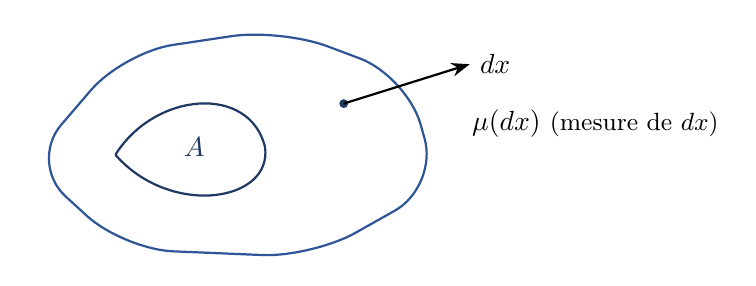
\begin{tikzpicture}[>=Stealth,thick]
  \draw[bleuclair,rounded corners=18pt] (0,0) -- (1.2,1.4) -- (3.2,1.7) -- (4.8,1.1) -- (5.2,-0.3) -- (3.6,-1.2) -- (1.2,-1.1) -- cycle;
  \draw[bleu] (1.1,0.1) .. controls (1.6,0.9) and (2.8,1.0) .. (3.0,0.2) .. controls (3.1,-0.5) and (1.8,-0.7) .. (1.1,0.1);
  \node[bleu] at (2.1,0.2) {$A$};
  \fill[bleu] (4.0,0.75) circle (1.6pt);
  \draw[->] (4.0,0.75) -- (5.6,1.25) node[right] {$dx$};
  \node[right] at (5.5,0.5) {$\mu(dx)$ \small(mesure de $dx$)};
\end{tikzpicture}
\end{center}

Pour $A\subset E$ :
\[
  \mu(A)=\int_A\mu(dx)=\int_A d\bigl(\mu(x)\bigr)=\int_E\ind_A\,d\mu(x)=\mu(A).
\]

\subsection*{Mesure de probabilité}

Soit $\mu:\Ff\to\Rb_+$ une mesure finie ($A\subset E$ ; $\mu(A)\le\mu(E)$, $\mu\ge0$). On définit
\[
  \PP:\ A\longmapsto\frac{\mu(A)}{\mu(E)} .
\]

%=====================================================================
\section*{Propriétés de continuité des probabilités}

Soit $(A_i)$ une suite d'événements et $B_i\subset A_i$ ; alors
\[
  \PP\Bigl(\bigcup A_i\Bigr)=\PP\Bigl(\bigcup B_i\Bigr)=\sum\PP(B_i)=\lim_{n\to+\infty}\sum_{i=1}^{n}\PP(B_i)\ \le\ \lim\sum_{i=1}^{n}\PP(A_i)=\sum\PP(A_i),
\]
puisque $\PP(B_i)\le\PP(A_i)$.

\textbf{\color{bleu}P6)} $(A_i)_{i\ge1}\nearrow$, c'est-à-dire $A_i\subset A_{i+1}$.
\[
  B_i=A_i\setminus\Bigl(\bigcup_{k<i}A_k\Bigr).
\]
$B_1=A_1$, $B_2=A_2\setminus A_1$, $B_1\cup B_2=A_1\cup(A_2\setminus A_1)=A_2$, \dots, $B_1\cup\dots\cup B_n=A_n$.
\[
  A_n=\bigcup_{i=1}^{n}B_i,\qquad \bigcup_{n\in\N}A_n=\bigcup_{n\in\N}\bigcup_{i=1}^{n}B_i=\bigcup_{i}B_i .
\]

Posons $B_1=A_1$, $B_i=A_i\cap\Bigl(\bigcup_{k\le i-1}A_k\Bigr)^c$.\\
$B_2=A_2\cap A_1^c$, \quad $B_3=A_3\cap(A_1\cup A_2)^c$.

\textbf{Montrons que les $B_i$ sont deux à deux disjoints.} Soit $i\neq j$ ; sans perte de généralité, $i<j$, c'est-à-dire $i\le j-1$.
\[
  B_j=A_j\cap\Bigl(\bigcup_{k=1}^{j-1}A_k\Bigr)^c,\qquad B_i=A_i\cap\Bigl(\bigcup_{l=1}^{i-1}A_l\Bigr)^c .
\]
Comme $i\le j-1$ : $A_i\subset A_{j-1}$, donc $A_i\cap A_{j-1}^c=\varnothing$. Alors
\[
  B_i\cap B_j=A_i\cap\Bigl(\bigcup_{k<i}A_k\Bigr)^c\cap A_j\cap\Bigl(\bigcap_{\substack{l<j\\ l\neq j-1}}A_l^c\Bigr)\cap A_{j-1}^c=\varnothing .
\]

\[
  B_1\cup B_2=A_1\cup[A_2\cap A_1^c]=(A_1\cup A_2)\cap\underbrace{(A_1\cup A_1^c)}_{=\Omega}=A_1\cup A_2 ,
\]
\[
  B_1\cup B_2\cup B_3=(A_1\cup A_2)\cup\bigl[A_3\cap(A_1\cup A_2)^c\bigr]
  =(A_1\cup A_2\cup A_3)\cap\bigl((A_1\cup A_2)\cup(A_1\cup A_2)^c\bigr)=A_1\cup A_2\cup A_3 .
\]

On a montré que $\displaystyle\bigcup A_i=\bigcup B_i$ avec $B_i\cap B_j=\varnothing$. Donc
\[
  \PP\Bigl(\bigcup A_i\Bigr)=\PP\Bigl(\bigcup B_i\Bigr)=\sum_{i=1}^{\infty}\PP(B_i)=\lim_{n\to+\infty}\sum_{i=1}^{n}\PP(B_i)
  =\lim_{n\to+\infty}\PP\Bigl(\bigcup_{i=1}^{n}B_i\Bigr)=\lim_{n\to+\infty}\PP(A_n).
\]

\textbf{\color{bleu}P7)} Soit $(A_i)\searrow$, c'est-à-dire $A_{i+1}\subset A_i\Rightarrow A_i^c\subset A_{i+1}^c\Rightarrow\{A_i^c\}\nearrow$, d'où
\[
  \PP\Bigl(\bigcup A_i^c\Bigr)=\lim_{n\to+\infty}\PP(A_n^c).
\]
Donc
\[
  \PP\Bigl[\Bigl(\bigcap A_i\Bigr)^c\Bigr]=1-\lim\PP(A_n),\qquad\text{et}\qquad 1-\PP\Bigl(\bigcap A_i\Bigr)=1-\lim\PP(A_i),
\]
soit $\PP\bigl(\bigcap A_i\bigr)=\lim\PP(A_i)$.

%=====================================================================
\section*{Mesure image}

Soit $T:(E,\Ff)\to(E',\Ff')$ mesurable et $\mu:\Ff\to\Rb_+$ une mesure.
\[
  \mu:\ \Ff\longrightarrow\Rb_+,\qquad A\longmapsto\mu(A),
\]
\[
  \mu_T:\ \Ff'\longrightarrow\Rb_+,\qquad A\longmapsto\mu_T(A)=\mu\bigl(T^{-1}(A)\bigr).
\]

\begin{note}
Le manuscrit s'arrête à « $\mu_T(A)=\mu($ » ; la définition est complétée par celle du cours de mesure.
\end{note}

%=====================================================================
\section*{Fonction de répartition}

\textbf{\color{bleu}$\ast$ Croissance.} Soit $x,y\in\R$ tels que $x\le y$. Montrons que $F_X(x)\le F_X(y)$.

On a : $F_X(x)=\PP(X\le x)$ et
\[
  (X\le x)=\{\omega\in\Omega\ /\ X(\omega)\le x\}\subset\{\omega\in\Omega\ /\ X(\omega)\le y\}\quad\text{car }x\le y .
\]
$\PP(X\le x)\le\PP(X\le y)$, donc $F_X(x)\le F_X(y)$.

\medskip
\textbf{\color{bleu}4)} \quad $\displaystyle\lim_{x\to-\infty}F_X(x)=\lim_{n\to+\infty}F_X(-n)$
\begin{align*}
  &=\lim_{n\to+\infty}\PP(X\le-n)=\lim_{n\to+\infty}\PP\bigl(X^{-1}(]-\infty;-n])\bigr)=\lim_{n\to+\infty}\PP_X\bigl(\underbrace{]-\infty;-n]}_{A_n}\bigr)\\
  &=\lim_{n\to+\infty}\PP(A_n)\ \text{ avec }(A_n)\searrow\\
  &=\PP_X\Bigl(\bigcap A_n\Bigr)=\PP_X(\varnothing)=\PP_X\bigl(X^{-1}(\varnothing)\bigr)=\PP(\varnothing)=0 .
\end{align*}

\begin{center}
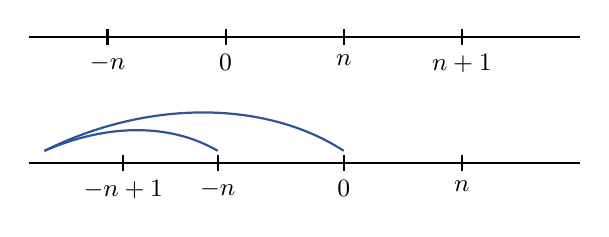
\begin{tikzpicture}[>=Stealth,thick,x=1cm,y=1cm]
  \draw (0,0) -- (7,0);
  \foreach \x/\l in {1/$-n$,2.5/$0$,4/$n$,5.5/$n+1$} {\draw (\x,0.1) -- (\x,-0.1) node[below,font=\small] {\l};}
  \begin{scope}[yshift=-1.6cm]
  \draw (0,0) -- (7,0);
  \foreach \x/\l in {1.2/$-n+1$,2.4/$-n$,4/$0$,5.5/$n$} {\draw (\x,0.1) -- (\x,-0.1) node[below,font=\small] {\l};}
  \draw[bleuclair] (0.2,0.15) .. controls (1.5,0.8) and (3,0.8) .. (4,0.15);
  \draw[bleuclair] (0.2,0.15) .. controls (1.0,0.5) and (1.8,0.5) .. (2.4,0.15);
  \end{scope}
\end{tikzpicture}
\end{center}

\textbf{\color{bleu}2) Continuité à droite.}
On veut montrer que $\displaystyle\lim_{x\to x_0^+}F_X(x)=F_X(x_0)$. On a :
\begin{align*}
  \lim_{x\to x_0^+}F_X(x)&=\lim_{n\to+\infty}F_X\Bigl(x_0+\frac1n\Bigr)\\
  &=\lim_{n\to+\infty}\PP\Bigl(X\le x_0+\frac1n\Bigr)=\lim_{n\to+\infty}\PP\Bigl(X^{-1}\bigl(]-\infty;x_0+\tfrac1n]\bigr)\Bigr)\\
  &=\lim_{n\to+\infty}\PP_X\Bigl(]-\infty;x_0+\tfrac1n]\Bigr).
\end{align*}
$n<n+1\Rightarrow\dfrac1{n+1}<\dfrac1n\Rightarrow A_{n+1}\subset A_n$ et $A_n\searrow$ :
\[
  =\PP_X\Bigl(\bigcap_{n}\,]-\infty;x_0+\tfrac1n]\Bigr).
\]
Soit $x\in\bigcap_n\,]-\infty;x_0+\frac1n]\Rightarrow\forall n$, $x\le x_0+\frac1n$. En passant à la limite, on a : $x\le x_0\Rightarrow x\in\,]-\infty;x_0]$.
Si $x\in\,]-\infty;x_0]$, $x\le x_0$ or $x_0\le x_0+\frac1n$ $\forall n$.

Donc $\displaystyle\bigcap_{n}\,]-\infty;x_0+\tfrac1n]=\,]-\infty;x_0]$.
\[
  \lim_{x\to x_0^+}F_X(x)=\PP_X\Bigl(\bigcap_n\,]-\infty;x_0+\tfrac1n]\Bigr)=\PP_X\bigl(]-\infty;x_0]\bigr)=\PP(X\le x_0)=F_X(x_0).
\]

\subsection*{Probabilité d'un intervalle}

$\blacksquare$\quad $\PP(a\le X<b)\neq\PP(a<X\le b)\neq\PP(a\le X\le b)$

\textit{Preuve.}

\underline{Cas 1 :} $\PP(a<X\le b)=F_X(b)-F_X(a)$.

\begin{center}
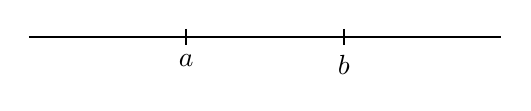
\begin{tikzpicture}[thick]
  \draw (0,0) -- (6,0);
  \draw (2,0.1) -- (2,-0.1) node[below] {$a$};
  \draw (4,0.1) -- (4,-0.1) node[below] {$b$};
\end{tikzpicture}
\end{center}

$]a,b]=\,]-\infty;b]\setminus\,]-\infty;a]$.
\begin{align*}
  \PP(a<X\le b)&=\PP_X\bigl(X^{-1}(]a,b])\bigr)=\PP_X(]a,b])\\
  &=\PP_X\bigl(]-\infty;b]\setminus\,]-\infty;a]\bigr)\\
  &=\PP_X(]-\infty;b])-\PP_X(]-\infty;a])\\
  &=\PP(X\le b)-\PP(X\le a)=F_X(b)-F_X(a).
\end{align*}

\underline{Cas 2 :} $\PP(a\le X<b)$. $\ [a,b[\,=\,]-\infty;b[\setminus\,]-\infty;a[$.
\begin{align*}
  \PP(a\le X<b)&=\PP_X([a,b[)\\
  &=\PP_X\bigl(]-\infty;b[\setminus\,]-\infty;a[\bigr)\\
  &=\PP_X(]-\infty;b[)-\PP_X(]-\infty;a[)\\
  &=\PP(X<b)-\PP(X<a)\\
  &=\lim_{x\to b^-}F_X(x)-\lim_{x\to a^-}F_X(x).
\end{align*}

%=====================================================================
\section*{Convergence d'une variable aléatoire}

\textbf{Pb :} On veut justifier le passage suivant
\[
  \lim_{n\to+\infty}\EE\bigl[f(X_n)\bigr]=\EE\Bigl(\lim_{n\to+\infty}f(X_n)\Bigr).
\]

\textbf{\color{bleu}Rappels :} notion de convergence de la V.A.

En $\R$ : $u_n\to u\iff\forall\varepsilon>0$, $\exists n_\varepsilon\in\N$, $n\ge N_\varepsilon\Rightarrow|u_n-u|<\varepsilon$.

Si $\{X_n\}$ est une suite de V.A, alors comment comprendre $X_n\to X$ ?

On pourrait penser à écrire
\[
  X_n\to X\ \text{ ssi }\ \forall\varepsilon>0,\ \exists n_\varepsilon\in\N\ /\ n\ge N_\varepsilon\Rightarrow|X_n-X|<\varepsilon .
\]
\textbf{Difficulté} (mode de convergence en probabilité) :
\begin{enumerate}[label=\textbf{\roman*)},leftmargin=1.2cm]
  \item $|X_n-X|$ est un évènement ;
  \item $|X_n-X|<\varepsilon\Rightarrow\{\omega\in\Omega\ /\ |X_n(\omega)-X(\omega)|<\varepsilon\}$ ;
  \item c'est un évènement et dire que $A_n$ se réalise avec une certaine probabilité.
\end{enumerate}

\subsection*{1\textsuperscript{er} mode de convergence}

\begin{enonce}{Convergence}{en probabilité}
\[
  X_n\xrightarrow{\ \PP\ }X\iff\forall\varepsilon>0,\ \exists n_\varepsilon\in\N,\quad n\ge N_\varepsilon\Rightarrow\PP(|X_n-X|<\varepsilon)\to1 .
\]
\end{enonce}

Comme $\PP(|X_n-X|<\varepsilon)=1-\PP(|X_n-X|\ge\varepsilon)$, on a de façon équivalente :
\[
  X_n\xrightarrow{\ \PP\ }X\iff\forall\varepsilon>0,\ \lim_{n\to+\infty}\PP(|X_n-X|>\varepsilon)=0 .
\]

\subsection*{2\textsuperscript{ème} mode (convergence presque sûre)}

\[
  X_n\xrightarrow{\ \text{p.s}\ }X\ \text{ ssi }\ \PP\bigl(\lim X_n=X\bigr)=1
\]
ssi $\exists\,\Omega_1\subset\Omega$ tel que $\PP(\Omega_1)=1$ et $\forall\omega_0\in\Omega_1$, $\displaystyle\lim_{n\to+\infty}X_n(\omega_0)=X(\omega_0)$.

Avec $\PP(\Omega\setminus\Omega_1)=0$ et $\forall\omega_0\in\Omega\setminus\Omega_1$, $\displaystyle\lim_{n\to+\infty}X_n(\omega_0)\neq X(\omega_0)$ (ou la limite n'existe pas).

\subsection*{3\textsuperscript{ème} mode (convergence en distribution)}

Soit $(X_n)$ une suite de V.A de fonction de répartition $F_{X_n}$.
\[
  X_n\xrightarrow{\ d\ }X\iff F_{X_n}(x)\longrightarrow F_X(x),\qquad\forall x\in F_X^{\,c}\ \ (\text{point de continuité de }F_X).
\]

%=====================================================================
\section*{Lois limites}

\textbf{\color{bleu}$\bullet$ LFGN} (loi faible des grands nombres). Si $(X_i)$ est une suite de V.A telle que $\EE(X_1)<+\infty$ et les $X_i$ sont iid, i.e.\ $\mu=\EE(X)$, $\sigma^2=\Var(X)$.
Alors
\[
  \frac1n\sum X_i\xrightarrow{\ \PP\ }\EE(X_1).
\]

\textbf{\color{bleu}$\bullet$ LPGN} (loi forte des grands nombres). $(X_i)$ iid telle que $\EE(X_i^{+})<+\infty$, $\mu=\EE(X_i)$, $\sigma^2=\Var(X_i)$ ; alors
\[
  \frac1n\sum X_i\xrightarrow{\ \text{p.s}\ }\EE(X_1).
\]

\textbf{\color{bleu}$\bullet$ TCL.} Si on a $(X_i)$ iid de moyenne $\mu=\EE(X_i)$, $\sigma^2=\Var(X_i)$ :
\[
  \sqrt n\,(\overline X_n-\mu)\xrightarrow{\ d\ }\mathcal N(0,\sigma^2).
\]
De même,
\[
  \frac{\sqrt n\,(\overline X_n-\mu)}{\sigma}\xrightarrow{\ d\ }\mathcal N(0,1),\qquad\text{où }\ \overline X_n=\frac1n\sum_{i=1}^{n}X_i .
\]

\begin{note}
La page « Lois limites » n'est reliée aux autres par aucune phrase ; elle est placée après les trois modes de convergence, dont elle utilise les notations.
\end{note}

%=====================================================================
\section*{Passage de la limite dans l'espérance}

On veut répondre à la question du passage de la limite dans l'espérance.

\textbf{3 résultats principaux :}
\begin{enumerate}[label=\textbf{(\roman*)},leftmargin=1.2cm]
  \item Beppo-Levi ;
  \item Convergence dominée ;
  \item Lemme de Fatou.
\end{enumerate}

\textbf{(i)} Si $X_n\nearrow$ ou $X_n\searrow$ tel que $X_n\to X$, on montre que (B.~Levi)
\[
  \lim_{n\to+\infty}\EE\bigl(f(X_n)\bigr)=\EE\bigl(\lim_n f(X_n)\bigr).
\]

\textbf{(ii) \underline{Convergence dominée.}} Soit $(X_n)_n$ une suite de V.A telle que $X_n\to X$ et il existe $Y$ tel que $|X_n|\le Y$ avec $Y\in L^1$
(espérance de valeur absolue est finie). Alors
\[
  \lim\EE\bigl(f(X_n)\bigr)=\EE\bigl(\lim f(X_n)\bigr).
\]

\begin{note}
Le lemme de Fatou (iii) est annoncé mais n'est pas développé dans le manuscrit.
\end{note}

%=====================================================================
\section*{Inégalité de Markov}

Soit $A\subset\Omega$ ; $\ind_A=\begin{cases}1&\text{si }x\in A\\0&\text{sinon}\end{cases}$, $\ \ind_\Omega=1$ \qquad(l'indicatrice est positive).

Soit $X$ une V.A positive et $a>0$.
\[
  X=X\times1=X\ind_\Omega .
\]
$\Omega=\{X<a\}\cup\{X\ge a\}$, donc
\[
  \ind_\Omega=\ind_{\{X<a\}}+\ind_{\{X\ge a\}},
\]
\[
  X\ind_\Omega=\underbrace{X\ind_{\{X<a\}}}_{\ge0}+X\ind_{\{X\ge a\}} .
\]
$X\ind_\Omega\ge X\ind_{\{X\ge a\}}$.
\[
  X\ge X\ind_{\{X\ge a\}}\ge a\ind_{\{X\ge a\}}\ \Longrightarrow\ X\ge a\ind_{\{X\ge a\}} .
\]

\textbf{Rappel :} (lien entre $\EE$ et $\PP$)
\[
  \PP(A)=\int_A d\PP=\int_\Omega\ind_A\,d\PP=\EE[\ind_A].
\]

D'où
\[
  X\ge a\ind_{\{X\ge a\}}\Rightarrow\EE(X)\ge a\,\EE\bigl(\ind_{\{X\ge a\}}\bigr)\Rightarrow\EE(X)\ge a\,\PP(X\ge a).
\]

\begin{enonce}{Inégalité}{de Markov}
\[
  \PP(X\ge a)\le\frac{\EE(X)}{a}.
\]
\end{enonce}

Si $X$ est une V.A quelconque, on pose $Y=|X|\ge0$, $a>0$ :
\[
  \PP(|X|\ge a)\le\frac{\EE|X|}{a},\qquad\PP(X^2\ge a^2)\le\frac{\EE(X^2)}{a^2}.
\]

Soit $X$ une V.A telle que $\EE(X)=\mu$ et $\Var(X)=\sigma^2$.
$Y=|X-\EE(X)|$.
\[
  \PP\bigl(|X-\EE(X)|\ge a\bigr),\ a>0\ =\ \PP\bigl(|X-\EE(X)|^2\ge a^2\bigr)\ \le\ \frac{\EE\bigl(|X-\EE(X)|^2\bigr)}{a^2}=\frac{\Var(X)}{a^2}=\frac{\sigma^2}{a^2}.
\]

\begin{note}
Le manuscrit alterne les écritures $\{X>a\}$ et $\{X\ge a\}$ ; j'ai uniformisé avec $\{X\ge a\}$, forme usuelle de l'inégalité de Markov. La mention « $\mu=\PP$ » écrite dans l'en-tête de la feuille n'est pas transcrite.
\end{note}

%=====================================================================
\section*{Inégalité de Cauchy-Schwarz}

\[
  \Bigl|\sum u_iv_i\Bigr|\le\sqrt{\Bigl(\sum u_i^2\Bigr)\Bigl(\sum v_i^2\Bigr)}.
\]
Soit $X,Y$ deux variables aléatoires.
\[
  \int|X|\cdot|Y|\,d\PP\le\sqrt{\int X^2\,d\PP\cdot\int Y^2\,d\PP}.
\]
Mieux encore,
\[
  \int|X-\EE(X)|\,|Y-\EE(Y)|\,d\PP\le\sqrt{\int\bigl(X-\EE(X)\bigr)^2d\PP}\times\sqrt{\int\bigl(Y-\EE(Y)\bigr)^2d\PP}
\]
\[
  \EE\bigl[|X-\EE(X)|\,|Y-\EE(Y)|\bigr]\le\sqrt{\Var(X)\Var(Y)}
\]
\[
  |\Cov(X,Y)|\le\sqrt{\Var(X)\Var(Y)},\qquad\Biggl|\frac{\Cov(X,Y)}{\sqrt{\Var(X)\Var(Y)}}\Biggr|\le1 .
\]

%=====================================================================
\section*{Paramètre de position}

On se place sur $(\Omega,\A,\PP)$. $X:\Omega\to\R$,
\[
  \EE(X)=\EE_{\PP}(X)=\int_\Omega X\,d\PP .
\]
Théorème de transfert : $\displaystyle\EE(X)=\int_\Omega X\,d\PP=\int_\R x\,d\PP_X(x)$.

On montre que
\[
  \mu_X=\argmin_{c\in\R}\ \EE\bigl[(X-c)^2\bigr].
\]
On pose $\varphi(c)=\EE\bigl[(X-c)^2\bigr]$
\begin{align*}
  &=\EE\bigl(X^2-2cX+c^2\bigr)\\
  &=\EE(X^2)-2c\,\EE(X)+c^2 ,
\end{align*}
$\varphi'(c)=-2\,\EE(X)+2c$, $\ \varphi''(c)=2>0$,\\
$\varphi'(c)=0\iff c=\EE(X)$.

\begin{note}
La page est photographiée en travers dans l'original ; elle a été redressée dans le PDF réorganisé.
\end{note}

\newpage
%=====================================================================
\section*{Inverse généralisée d'une fonction de répartition}

Soit $q\in\,]0,1[$ :
\[
  F^{(-1)}(q)=\inf\bigl\{x\in\R,\ F(x)\ge q\bigr\}.
\]

\begin{note}
Le titre de cette section est de moi ; le manuscrit commence directement par la définition. Il écrit tantôt $F^{-1}$, tantôt $F^{(-1)}$ pour l'inverse généralisé :
j'écris toujours $F^{(-1)}$ et je réserve $F^{-1}$ à la bijection réciproque du cas (P1). Les énoncés de (P1), (P2), (P3) ne sont pas écrits dans le cahier ;
je les déduis de leurs preuves.
\end{note}

\textbf{\color{bleu}(P1)} \textit{Si $F$ est une bijection, $F^{(-1)}=F^{-1}$.}

\textit{Preuve (P1).} Si $F$ est bijective (continue et strictement croissante) :

\begin{center}
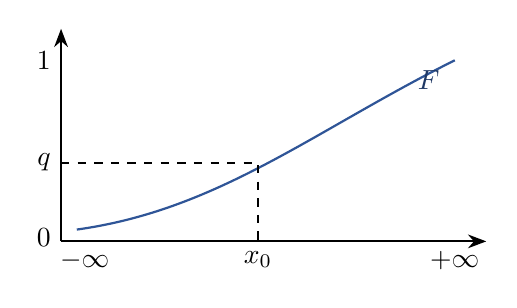
\begin{tikzpicture}[>=Stealth,thick,x=1cm,y=1cm]
  \draw[->] (0,0) -- (5.4,0);
  \draw[->] (0,0) -- (0,2.7);
  \draw[bleuclair] (0.2,0.15) .. controls (2,0.4) and (3.2,1.4) .. (5,2.3);
  \draw[dashed] (0,1.0) -- (2.5,1.0) -- (2.5,0);
  \node[left] at (0,1.0) {$q$};
  \node[left] at (0,2.3) {$1$};
  \node[left] at (0,0.05) {$0$};
  \node[below] at (2.5,0) {$x_0$};
  \node[below] at (0.3,0) {$-\infty$};
  \node[below] at (5.0,0) {$+\infty$};
  \node[right,bleu] at (4.4,2.05) {$F$};
\end{tikzpicture}
\end{center}

Si $q\in\,]0,1[$, $\exists!\,x_0\in\R$ tel que $F(x_0)=q$, c'est-à-dire $x_0=F^{-1}(q)$. Donc
\[
  \{x\in\R,\ F(x)\ge q\}=[F^{-1}(q),+\infty[\,.
\]
Ainsi $\inf\{x\in\R,\ F(x)\ge q\}=F^{-1}(q)$, d'où $F^{(-1)}(q)=F^{-1}(q)$.

\medskip
\textbf{\color{bleu}(P2)} \textit{$F^{(-1)}$ est croissante.}

\textit{Preuve (P2).} Soit $q_1,q_2\in\,]0,1[$ tels que $q_1\le q_2$. Alors
\[
  \{x\in\R,\ F(x)\ge q_2\}\subset\{x\in\R,\ F(x)\ge q_1\}.
\]
Donc
\[
  \inf\{x\in\R,\ F(x)\ge q_2\}\ \ge\ \inf\{x\in\R,\ F(x)\ge q_1\},
\]
d'où $F^{(-1)}(q_2)\ge F^{(-1)}(q_1)$.

\medskip
\textbf{N.B.} Avant la preuve (P3) on a le lemme suivant.

\begin{enonce}{Lemme}{}
Si $q\in\,]0,1[$ on a toujours $F\bigl(F^{(-1)}(q)\bigr)\ge q$.
\end{enonce}

\textit{Preuve.} Par caractérisation de l'inf, on a :

\begin{center}
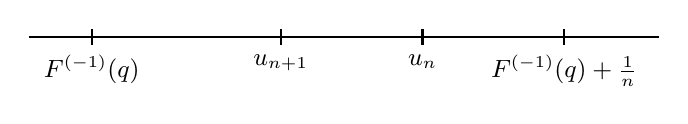
\begin{tikzpicture}[thick,>=Stealth]
  \draw (0,0) -- (8,0);
  \foreach \x/\l in {0.8/$F^{(-1)}(q)$,3.2/$u_{n+1}$,5.0/$u_n$,6.8/$F^{(-1)}(q)+\frac1n$} {\draw (\x,0.1) -- (\x,-0.1) node[below,font=\small] {\l};}
\end{tikzpicture}
\end{center}

$\forall n\ge1$, $\exists u_n$ tel que $F(u_n)\ge q$ qui vérifie
\[
  F^{(-1)}(q)\le u_n\le F^{(-1)}(q)+\frac1n .
\]
$F$ étant croissante :
\[
  F\Bigl(F^{(-1)}(q)+\frac1n\Bigr)\ge F(u_n)\ge q .
\]
En passant à la limite et en se servant du fait que $F$ est continue à droite, on a :
\[
  \lim_{n\to+\infty}F\Bigl(F^{(-1)}(q)+\frac1n\Bigr)\ge q,
\]
donc $F\bigl(F^{(-1)}(q)\bigr)\ge q$.

\begin{note}
Le schéma de droite (points $u_n$, $u_{n+1}$ et bornes de l'intervalle) est peu lisible dans le cahier ; je le redessine de façon schématique. Le N.B. annonce le lemme « avant la preuve (P2) » ;
c'est (P3) qui l'utilise (voir plus bas), je lis donc (P3).
\end{note}

\medskip
\textbf{\color{bleu}(P3)} \textit{$\forall x\in\R$, $\forall q\in\,]0,1[$ : $F(x)\ge q\iff x\ge F^{(-1)}(q)$.}

\textit{Preuve (P3).} $\forall x\in\R$, $\forall q\in\,]0,1[$ :
\[
  F(x)\ge q\iff x\ge F^{(-1)}(q).
\]
$(\Rightarrow)$ Si $F(x)\ge q$ alors $x\in\{y\in\R,\ F(y)\ge q\}$, donc
\[
  x\ge\inf\{y\in\R,\ F(y)\ge q\}=F^{(-1)}(q),
\]
d'où $x\ge F^{(-1)}(q)$.

$(\Leftarrow)$ Supposons $x\ge F^{(-1)}(q)$. $F$ étant croissante, $F(x)\ge F\bigl(F^{(-1)}(q)\bigr)$. Or le lemme prouvé entraîne $F\bigl(F^{(-1)}(q)\bigr)\ge q$, d'où $F(x)\ge q$.

%=====================================================================
\section*{Caractérisation du quantile}

\begin{enonce}{Définition}{(caractérisation du quantile)}
Soit $q_\beta$, $\beta\in\,]0,1[$, on a toujours
\[
  \PP(X\ge q_\beta)\ge1-\beta\qquad\text{et}\qquad\PP(X\le q_\beta)\ge\beta,
\]
où $q_\beta=\inf\{x\in\R,\ F(x)\ge\beta\}$.
\end{enonce}

\textit{Preuve.} En posant $u_n=q_\beta-\dfrac1n$, on a $u_n\nearrow$, $u_n<q_\beta$ et $u_n\to q_\beta$.
On pose ensuite $C_n=\{X\le u_n\}$.

\textbf{i)} Montrons que $\displaystyle\bigcup_nC_n=\{X<q_\beta\}$.

$(\Rightarrow)$ Soit $\omega\in\bigcup C_n$, c'est-à-dire $\exists n_0$ tel que $\omega\in C_{n_0}$ :
\[
  X(\omega)\le u_{n_0}<q_\beta\Rightarrow\omega\in\{X<q_\beta\}\Rightarrow\bigcup C_n\subset\{X<q_\beta\}.
\]
$(\Leftarrow)$ Soit $\omega\in\{X<q_\beta\}$, c'est-à-dire $X(\omega)<q_\beta$, c'est-à-dire $q_\beta-X(\omega)>0$.
$u_n\to q_\beta\Rightarrow$ pour $\varepsilon=q_\beta-X(\omega)$, $\exists n_\varepsilon\in\N$ tel que
\[
  n\ge n_\varepsilon\Rightarrow-\bigl(q_\beta-X(\omega)\bigr)\le u_n-q_\beta\le q_\beta-X(\omega),
\]
d'où
\[
  -q_\beta+X(\omega)\le u_n-q_\beta\Rightarrow X(\omega)\le u_n .
\]
C'est-à-dire $\exists n_0$ tel que $n\ge n_0$, $X(\omega)\le u_n$, c'est-à-dire $\omega\in\displaystyle\bigcup_n\{X\le u_n\}$.

\textbf{ii)} On part du fait que $\bigcup C_n=\{X<q_\beta\}$. D'une part,
\begin{align*}
  \PP(X<q_\beta)&=\PP\Bigl(\bigcup_nC_n\Bigr)\\
  &=\lim_{n\to+\infty}\PP(C_n)\quad\text{car }C_n\nearrow\\
  &=\lim_{n\to+\infty}\PP\bigl(\{X\le u_n\}\bigr)=\lim_{n\to+\infty}\PP(X\le u_n)\\
  &=\lim_{n\to+\infty}F(u_n)\le\beta
\end{align*}
(car $u_n<q_\beta=\inf\{x\in\R,\ F(x)\ge\beta\}$, donc $F(u_n)<\beta$).

\textbf{N.B.} $q_\beta=\inf\{x,\ F(x)\ge\beta\}\Rightarrow\begin{cases}F(q_\beta)\ge\beta\\ \text{si }q^\circ<q_\beta\Rightarrow F(q^\circ)<\beta\end{cases}$

Pour avoir $F(q_\beta)=\beta$ il faut que $F^{(-1)}=F^{-1}$.

D'où $\PP(X<q_\beta)\le\beta$, donc
\[
  1-\PP(X<q_\beta)\ge1-\beta\ \Rightarrow\ \PP(X\ge q_\beta)\ge1-\beta .
\]
D'autre part,
\[
  \PP(X\le q_\beta)=F(q_\beta)=F\bigl(F^{(-1)}(\beta)\bigr)\ge\beta .
\]

\subsection*{Remarque importante (utilisée dans les IC et les tests)}

Si $X$ est une v.a. et $q_\alpha$, $q_{\alpha'}$ sont des quantiles associés tels que $q_\alpha<q_{\alpha'}$, alors
\begin{align*}
  \PP(q_\alpha\le X\le q_{\alpha'})&=F(q_{\alpha'})-\PP(X<q_\alpha)\\
  &\ge\alpha'-\bigl(1-\PP(X\ge q_\alpha)\bigr)\\
  &\ge\alpha'-1+\PP(X\ge q_\alpha)\\
  &\ge\alpha'-1+1-\alpha\\
  &\ge\alpha'-\alpha .
\end{align*}
Donc $\PP(q_\alpha\le X\le q_{\alpha'})\ge\alpha'-\alpha$.

En particulier si $\alpha'=1-\dfrac\beta2$ et $\alpha=\dfrac\beta2$ :
\[
  \PP\bigl(q_{\beta/2}\le X\le q_{1-\beta/2}\bigr)\ge1-\beta .
\]

\begin{note}
Le manuscrit écrit $\PP(q_\alpha<X\le q_{\alpha'})=F(q_{\alpha'})-F(q_\alpha)$, et de même $q_{\beta/2}<X<q_{1-\beta/2}$ à la fin ; mais la minoration qui suit utilise $\PP(X<q_\alpha)=1-\PP(X\ge q_\alpha)$ à la place de $F(q_\alpha)=\PP(X\le q_\alpha)$.
Les deux ne coïncident que si $\PP(X=q_\alpha)=0$ ; j'ai donc écrit l'énoncé exact (inégalités larges), qui est celui que la suite des calculs démontre.
\end{note}

%=====================================================================
\section*{Espérance conditionnelle}

Soit $X,Y$ deux v.a. On veut donner un sens à $\EE[X\mid Y]$. On se place dans le cas discret :
$\EE[X\mid Y=y]=\;?$

\begin{align*}
  \EE\bigl[X\mid\underbrace{\{Y=y\}}_{\text{évènement}}\bigr]&=\sum_xx\,\PP(X=x\mid Y=y)\\
  &=\sum_xx\,\frac{\PP(X=x,\,Y=y)}{\PP(Y=y)}\\
  &=\frac1{\PP(Y=y)}\sum_xx\,\EE\bigl[\ind_{\{X=x\}\cap\{Y=y\}}\bigr]\\
  &=\frac1{\PP(Y=y)}\,\EE\Bigl[\sum_xx\,\ind_{\{X=x\}}\ind_{\{Y=y\}}\Bigr].
\end{align*}

\textbf{Remarque :} $\displaystyle\sum_xx\,\ind_{\{X=x\}}=X$.
Soit $\omega\in\Omega$, $\exists x_0$ tel que $X(\omega)=x_0$ :
\[
  \sum_xx\,\ind_{\{X=x\}}(\omega)=\sum_xx\,\ind_{\{X(\omega)=x\}}=x_0=X(\omega).
\]
$\Rightarrow\ \EE[X\mid Y=y]=\dfrac1{\PP(Y=y)}\,\EE\bigl(X\ind_{\{Y=y\}}\bigr)$.

De façon générale, on définit pour tout évènement $B$ :
\begin{equation*}
  \EE(X\mid B)=\frac1{\PP(B)}\,\EE(X\ind_B).\tag{1}
\end{equation*}
Si on se rappelle sur $(\Omega,\Ff,\PP)$ que $\EE(X)=\displaystyle\int_\Omega X\,d\PP$, en passant à l'espérance sur (1), on a :

\textbf{Rappel :} $\displaystyle\int_Bf(x)\ind_A\,dx=\int_{A\cap B}f(x)\,dx$.
\begin{align*}
  \int_\Omega\EE(X\mid B)\,d\PP&=\frac1{\PP(B)}\int_\Omega\EE(X\ind_B)\,d\PP\\
  &=\frac1{\PP(B)}\,\EE\Bigl[\int_\Omega X\ind_B\,d\PP\Bigr]\\
  &=\frac1{\PP(B)}\,\EE\Bigl[\int_BX\,d\PP\Bigr].
\end{align*}
Pour $B=\Omega$, $\ \EE\bigl(\EE(X\mid\Omega)\bigr)=\EE(X)$.

\begin{note}
Le calcul de $\int_\Omega\EE(X\mid B)\,d\PP$ est transcrit tel quel ; il n'est pas conclu dans le cahier, qui passe directement au cas $B=\Omega$. Le libellé exact du « Rappel » (numéro) est peu lisible ; je ne le reproduis pas.
\end{note}

\begin{enonce}{Définition}{(espérance conditionnelle)}
Soit $\mathscr G\subset\Ff$ une tribu contenue dans $\Ff$. On appelle $\EE(X\mid\mathscr G)$ l'unique v.a. $\mathscr G$-mesurable et qui vérifie : $\forall Z$ $\mathscr G$-mesurable, on a toujours
\[
  \EE\bigl(Z\,\EE(X\mid\mathscr G)\bigr)=\EE(XZ).
\]
\end{enonce}

Pour donner un sens à $\EE(X\mid Y)$ on écrit $\EE(X\mid Y):=\EE\bigl(X\mid\sigma(Y)\bigr)$ où $\sigma(Y)=\bigl\{Y^{-1}(A):A\in\B(\R)\bigr\}$.

\subsection*{Quelques propriétés}

\textbf{\color{bleu}P1)} $\EE\bigl(\EE(X\mid Y)\bigr)=\EE(X)$.

\textbf{\color{bleu}P2)} $\forall\alpha,\beta\in\R$,
\[
  \EE[\alpha X+\beta Y\mid Z]=\alpha\,\EE(X\mid Z)+\beta\,\EE(Y\mid Z).
\]
Posons $V=\alpha\,\EE(X\mid Z)+\beta\,\EE(Y\mid Z)$. Soit $T$ une v.a. $Z$-mesurable.
\[
  \EE[TV]=\EE\bigl(T(\alpha X+\beta Y)\bigr)\ \text{ à montrer :}
\]
\begin{align*}
  \EE(T\cdot V)&=\EE\bigl(T\cdot(\alpha\,\EE(X\mid Z)+\beta\,\EE(Y\mid Z))\bigr)\\
  &=\EE\bigl(T\cdot\alpha\,\EE(X\mid Z)+T\cdot\beta\,\EE(Y\mid Z)\bigr)\\
  &=\EE\bigl(T\alpha\,\EE(X\mid Z)\bigr)+\EE\bigl(T\beta\,\EE(Y\mid Z)\bigr)\\
  &=\EE(T\cdot\alpha X)+\EE(T\cdot\beta Y)\\
  &=\EE\bigl(T(\alpha X+\beta Y)\bigr).
\end{align*}

\begin{note}
La dernière ligne de la preuve de P2 est inachevée dans le manuscrit (« $=\EE(\alpha$ ») ; je la complète par $\EE\bigl(T(\alpha X+\beta Y)\bigr)$, qui est le terme à obtenir.
La phrase « Soit $T$ une v.a. $Z$-mesurable » est à demi barrée dans le cahier.
\end{note}

\textbf{\color{bleu}P3)} On part de ce qu'on connaît : si $X,Y$ sont deux v.a.,
\[
  \EE[XY\mid Y]=Y\,\EE(X\mid Y).
\]
De façon générale
\[
  \EE[X\,g(Y)\mid Y]=g(Y)\,\EE(X\mid Y).
\]

\textbf{\color{bleu}P4) Indépendance.} Si $X\perp\!\!\!\perp Y$, $\ \EE(X\mid Y)=\EE(X)$.

\textbf{\color{bleu}P5)} Si $\Ff_1\subset\Ff_2$ :
\begin{align*}
  \EE(X\mid\Ff_1)&=\EE\bigl(\EE(X\mid\Ff_2)\mid\Ff_1\bigr)\\
  &=\EE\bigl(\EE(X\mid\Ff_1)\mid\Ff_2\bigr),
\end{align*}
\begin{align*}
  \EE(X\mid\Ff_2)&=\EE\bigl(\EE(X\mid\Ff_2)\mid\Ff_2\bigr).
\end{align*}

\begin{note}
Les trois lignes de P5 sont difficiles à lire (les indices $1$ et $2$ se ressemblent et deux lignes semblent identiques). Je lis la propriété de la tour :
$\EE(X\mid\Ff_1)=\EE(\EE(X\mid\Ff_2)\mid\Ff_1)=\EE(\EE(X\mid\Ff_1)\mid\Ff_2)$, et $\EE(X\mid\Ff_2)$ est invariante par conditionnement par $\Ff_2$.
\end{note}

\textbf{\color{bleu}P6)}
\[
  \Var(X)=\Var\bigl(\EE(X\mid Y)\bigr)+\EE\bigl(\Var(X\mid Y)\bigr).
\]

\textbf{Remarque :}
$\begin{cases}\EE(X)=\text{cte}\\ \EE(X\mid Y)\text{ est une v.a.}\end{cases}$
\[
  \EE(X\mid Y):\ \Omega\longrightarrow\R,\qquad \omega\longmapsto\EE\bigl(X\mid Y=Y(\omega)\bigr).
\]

Commençons par définir $\Var(X\mid Y)=\;?$

On sait que
\[
  \Var(X)=\EE\bigl[(X-\EE(X))^2\bigr],\qquad
  \Var(X\mid Y)=\EE\bigl[\bigl((X\mid Y)-\EE(X\mid Y)\bigr)^2\bigr]
\]
(cette écriture de $\Var(X\mid Y)$ n'a pas de sens en probabilité).
On va donc remplacer $\EE\bigl[\bigl((X\mid Y)-\EE(X\mid Y)\bigr)^2\bigr]$ par $\EE\bigl[\bigl(X-\EE(X\mid Y)\bigr)^2\mid Y\bigr]$.

\begin{align*}
  \Var(X)&=\EE\bigl[(X-\EE(X))^2\bigr]\\
  &=\EE\bigl[\bigl(X-\EE(X\mid Y)+\EE(X\mid Y)-\EE(X)\bigr)^2\bigr]\\
  &=\EE\bigl[(X-\EE(X\mid Y))^2\bigr]+\EE\bigl[(\EE(X\mid Y)-\EE(X))^2\bigr]\\
  &\quad+2\,\EE\bigl[(X-\EE(X\mid Y))(\EE(X\mid Y)-\EE(X))\bigr]\\
  &=A+B+2C .
\end{align*}

\textbf{$\ast$ Analysons $A$ :}
\begin{align*}
  A&=\EE\bigl[(X-\EE(X\mid Y))^2\bigr]\\
  &=\EE\Bigl[\EE\bigl((X-\EE(X\mid Y))^2\mid Y\bigr)\Bigr]\\
  &=\EE\bigl[\Var(X\mid Y)\bigr].
\end{align*}

\textbf{$\ast$ Analysons $B$ :}
\begin{align*}
  B&=\EE\bigl[(\EE(X\mid Y)-\EE(X))^2\bigr]\\
  &=\EE\bigl[(\EE(X\mid Y)-\EE(\EE(X\mid Y)))^2\bigr]\\
  &=\Var\bigl(\EE(X\mid Y)\bigr)\qquad(\EE(X\mid Y)=\varphi(Y)).
\end{align*}

\textbf{Analysons $C$ :}
\begin{align*}
  C&=\EE\bigl[(X-\EE(X\mid Y))(\EE(X\mid Y)-\EE(X))\bigr]\\
  &=\EE\Bigl[\EE\bigl((X-\EE(X\mid Y))(\EE(X\mid Y)-\EE(X))\mid Y\bigr)\Bigr]\\
  &=\EE\Bigl[(\EE(X\mid Y)-\EE(X))\,\underbrace{\EE\bigl((X-\EE(X\mid Y))\mid Y\bigr)}_{\gamma}\Bigr],
\end{align*}
\begin{align*}
  \gamma&=\EE\bigl[(X-\EE(X\mid Y))\mid Y\bigr]\\
  &=\EE(X\mid Y)-\EE\bigl(\EE(X\mid Y)\mid Y\bigr)\\
  &=\EE(X\mid Y)-\EE(X\mid Y)\,\underbrace{\EE(1\mid Y)}_{1}\\
  &=0 .
\end{align*}
D'où
\[
  \boxed{\ \Var(X)=\Var\bigl(\EE(X\mid Y)\bigr)+\EE\bigl[\Var(X\mid Y)\bigr]\ }
\]

\begin{note}
Dans les deux premières lignes du calcul de $C$, le manuscrit semble écrire $\EE(Y)$ au lieu de $\EE(X)$ dans le second facteur ; comme $C$ est défini ci-dessus avec $\EE(X)$ et que le calcul ne dépend que de la $\sigma(Y)$-mesurabilité de ce facteur, je lis $\EE(X)$ partout.
\end{note}

\subsection*{Exercice}

Si $X\sim\mathcal U([a,b])$, $X\perp\!\!\!\perp Y$, $Y\sim\mathcal U([a,b])$. Calculer $\PP(X<Y)=\;?$

\subsection*{Pratique de $\EE(X\mid Y)$}

Se rappeler que, d'après le lemme de Doob, $\exists\varphi$ mesurable telle que $\EE(X\mid Y)=\varphi(Y)$.

En pratique, pour avoir $\EE(X\mid Y)$, on procède en deux étapes.

\textbf{i)} On calcule $\EE(X\mid Y=y)$, on obtient $\varphi(y)$.

\textbf{ii)} On déduit $\EE(X\mid Y)$ en remplaçant $y$ par $Y$ dans $\varphi(y)$.

Si $X,Y$ sont continues :
\[
  \EE(X\mid Y=y)=\int x\,f_{X\mid Y=y}(x)\,dx\qquad\text{où}\qquad f_{X\mid Y=y}(x)=\frac{f_{X,Y}(x,y)}{f_Y(y)} .
\]
Si $X$ et $Y$ sont discrètes,
\[
  \EE(X\mid Y=y)=\sum x\,\PP(X=x\mid Y=y)\qquad\text{où}\qquad\PP(X=x\mid Y=y)=\frac{\PP(X=x,\,Y=y)}{\PP(Y=y)} .
\]

\textbf{Solution de l'exercice.} On a :
\begin{align*}
  \PP(X<Y)&=\EE\bigl[\ind_{\{X<Y\}}\bigr]\\
  &=\EE\bigl[\EE\bigl(\ind_{\{X<Y\}}\mid Y\bigr)\bigr]\\
  &=\EE\bigl(\varphi(Y)\bigr)\quad\text{où}
\end{align*}
\begin{align*}
  \varphi(y)&=\EE\bigl(\ind_{\{X<Y\}}\mid Y=y\bigr)\\
  &=\EE\bigl(\ind_{\{X<y\}}\mid Y=y\bigr)\\
  &=\EE\bigl[\ind_{\{X<y\}}\bigr]\quad\text{car }X\perp\!\!\!\perp Y\\
  &=\PP(X<y)\\
  &=\int_a^y\frac1{b-a}\,dx\\
  &=\frac{y-a}{b-a}\,\ind_{[a,b]}(y)
\end{align*}
$\Rightarrow\ \varphi(y)=\dfrac{y-a}{b-a}$

$\Rightarrow\ \EE\bigl(\varphi(Y)\bigr)=\dfrac{\EE(Y)-a}{b-a}$.

Or $Y\sim\mathcal U([a,b])$, $\EE(Y)=\dfrac{a+b}2$, d'où
\[
  \EE\bigl(\varphi(Y)\bigr)=\frac{\frac{a+b}2-a}{b-a}=\frac12 .
\]
D'où $\PP(X<Y)=\dfrac12$.

\begin{note}
Dans la ligne $\varphi(y)=\frac{y-a}{b-a}\ind_{[a,b]}(y)$ l'indicatrice disparaît ensuite : c'est licite car $Y\in[a,b]$ presque sûrement.
\end{note}

%---------------------------------------------------------------------
\subsection*{Exercice 7}

Soient $X\sim\mathcal P(\lambda)$, $Y\sim\mathcal P(t)$ indépendantes. Montrer que $X+Y\sim\mathcal P(\lambda+t)$.

\begin{align*}
  \{X+Y=k\}&=(X+Y=k)\cap\Omega\\
  &=(X+Y=k)\cap\Bigl(\bigcup_i\{X=i\}\Bigr)\\
  &=\bigcup_i\,[X+Y=k,\ X=i].
\end{align*}
Ainsi
\begin{align*}
  \PP(X+Y=k)&=\sum_i\PP(X+Y=k,\ X=i)\\
  &=\sum_i\PP(X+Y=k\mid X=i)\,\PP(X=i)\\
  &=\sum_i\PP(Y=k-i\mid X=i)\,\PP(X=i)\\
  &=\sum_i\PP(Y=k-i,\ X=i)\\
  &=\sum_{\substack{i\\ k-i\ge0}}\PP(Y=k-i,\ X=i)+\sum_{\substack{i\\ k-i<0}}\PP(Y=k-i,\ X=i)\\
  &=\sum_{i=0}^{k}\PP(Y=k-i,\ X=i)\\
  &=\sum_{i=0}^{k}\PP(Y=k-i)\times\PP(X=i)\qquad\text{car }X\perp\!\!\!\perp Y\\
  &=\sum_{i=0}^{k}\frac{e^{-t}\,t^{k-i}}{(k-i)!}\times\frac{e^{-\lambda}\lambda^{i}}{i!}\\
  &=\frac{e^{-(\lambda+t)}}{k!}\sum_{i=0}^{k}C_k^i\,\lambda^it^{k-i}\\
  &=\frac{e^{-(\lambda+t)}\,(\lambda+t)^k}{k!}.\qquad\blacksquare
\end{align*}
D'où $X+Y\sim\mathcal P(\lambda+t)$.

\begin{note}
Dans l'avant-dernière étape de la première chaîne, la seconde somme (indices $i$ avec $k-i<0$) est nulle puisque $\PP(Y=k-i)=0$ pour $k-i<0$ ; elle disparaît dans la ligne suivante.
\end{note}

%---------------------------------------------------------------------
\subsection*{Exercice 11}

\begin{note}
Le manuscrit annonce « Exercice 11 : » en haut d'une page, mais l'énoncé n'est pas écrit (la page est vierge).
\end{note}

%=====================================================================
\newpage
\datepage{Lundi 19 octobre 2026}
\section*{Chapitre 2 : Concepts fondamentaux}

L'objectif de ce chapitre est de décrire le cadre mathématique dans lequel s'inscrit la démarche statistique.
Avant de présenter rigoureusement ce cadre, nous introduisons deux exemples motivants qui permettront de mieux appréhender les problématiques statistiques usuelles.

\subsection*{2.1) Exemples et problématiques}

\textbf{\color{bleu}Exemple 2.1} (Sondage d'opinion). Un projet de loi est soumis à un référendum. À cette occasion on interroge $n$ individus issus de la population camerounaise.
On note $X_i=1$ si le $i$-ème individu répond « oui » et $X_i=0$ s'il répond « non ».

En supposant que les individus sont choisis au hasard de manière indépendante, on modélise les variables aléatoires $X_1,\dots,X_n$ comme étant i.i.d.\ selon une loi de Bernoulli de paramètre $\theta$, $\mathcal B(\theta)$, $\theta\in\,]0,1[$.
Le paramètre $\theta$ représente la proportion théorique de citoyens favorables au projet de loi. À partir des données observées $(x_1,\dots,x_n)$ les objectifs sont :
\begin{itemize}
  \item Estimer la valeur du paramètre $\theta$.
  \item Tester si le projet de loi sera adopté, c'est-à-dire trancher entre les hypothèses $\theta>\frac12$ et $\theta\le\frac12$.
\end{itemize}

\textbf{\color{bleu}Exemple 2.2} (Modélisation du trafic téléphonique). Une entreprise de téléphonie souhaite modéliser le nombre journalier d'appels passés par ses clients à l'aide d'une loi de Poisson.
Cette modélisation lui est indispensable pour ajuster sa grille tarifaire.

Pour valider cette hypothèse, elle collecte le nombre d'appels effectués en une journée par un échantillon de $n$ clients choisis au hasard.
On dispose ainsi de l'observation de $n$ variables aléatoires $X_1,\dots,X_n$ de loi inconnue.

La démarche comporte deux étapes :
\begin{itemize}
  \item Tester si la loi sous-jacente des observations est effectivement une loi de Poisson.
  \item Estimer le paramètre $\theta$ ($\theta>0$) de cette loi si l'hypothèse est conservée.
\end{itemize}

L'objet de la statistique inférentielle est de répondre à ce type de questions. Contrairement à la théorie des probabilités où la loi des probabilités est supposée entièrement connue et où l'on étudie le comportement théorique des variables aléatoires, la statistique adopte la démarche inverse : à partir des observations d'un phénomène aléatoire, que peut-on déduire sur la loi des probabilités sous-jacente.

\textbf{\color{bleu}Remarque 2.1.} Un modèle statistique n'est qu'une idéalisation mathématique simplifiée de la réalité ; le choix d'un modèle repose à la fois sur une connaissance préalable du phénomène étudié, sur le protocole expérimental et sur l'analyse exploratoire (ou graphique).

%---------------------------------------------------------------------
\subsection*{2.2) Modélisation statistique}

\subsubsection*{a) Cadre statistique}

En statistique, on dispose d'un jeu d'observations numériques noté $x=(x_1,\dots,x_n)\in\R^n$.
On modélise ces observations comme la réalisation d'un vecteur aléatoire $X=(X_1,\dots,X_n)$ sur un espace probabilisé $(\Omega,\A,\PP)$ de telle sorte que :
\[
  \forall i\in\{1,\dots,n\},\quad X_i(\Omega)\subset\R\quad\text{et}\quad X_i(\omega)=x_i .
\]
En d'autres termes $x_i\in X_i(\Omega)$.

Selon le degré de connaissance de la loi commune des variables $X_i$, la statistique se divise en deux grands domaines :
\begin{itemize}
  \item \textbf{La statistique paramétrique :} la forme fonctionnelle de la loi $\mathcal L$ est connue à un paramètre $\theta$ près et dans ce cas l'inférence porte uniquement sur $\theta$.\\
        Si $\mathcal L=\mathcal B(p)$ alors $\theta=p$ ; si $\mathcal L=\mathcal N(m,\sigma^2)\Rightarrow\theta=(m,\sigma^2)$.
  \item \textbf{La statistique non paramétrique :} la loi $\mathcal L$ est complètement inconnue et on cherche à estimer les caractéristiques fonctionnelles globales telles que la densité $f$, la fonction de répartition ou la fonction caractéristique.
\end{itemize}

\subsubsection*{b) Notion de modèle statistique}

\begin{enonce}{Définition}{}
On appelle \emph{modèle statistique} la structure formée par un espace d'état (ou d'observation) $E$, une tribu $\Ee$ sur $E$ et une famille de mesures de probabilité $\mathscr P$ définie sur $(E,\Ee)$.
\end{enonce}

La vraie loi de probabilité $\PP$ régissant l'observation $x=(x_1,\dots,x_n)$ est inconnue mais on suppose qu'elle appartienne à la famille $\mathscr P$. (Le but est de trouver $\PP$.)

\textbf{Modèle paramétrique.} Un modèle statistique $(E,\Ee,\mathscr P)$ est dit \emph{paramétrique} s'il existe un ensemble $\Theta\subset\R^d$ appelé espace des paramètres et une application surjective
\[
  \Theta\longrightarrow\mathscr P,\qquad\theta\longmapsto P_\theta .
\]
On note alors la famille des lois $\mathscr P=\{P_\theta,\ \theta\in\Theta\}$ et le modèle statistique paramétrique sera donc $\bigl(E,\Ee,\{P_\theta\}_{\theta\in\Theta}\bigr)$.

\textbf{N.B.} Notons que la recherche des paramètres dans un modèle statistique n'est possible que si ce dernier est identifiable.

\begin{enonce}{Définition}{(identifiabilité)}
Un modèle statistique paramétrique est dit \emph{identifiable} si l'application $\theta\mapsto P_\theta$ est injective. En d'autres termes
\[
  \forall\theta_1,\theta_2\in\Theta,\qquad\theta_1\neq\theta_2\Rightarrow P_{\theta_1}\neq P_{\theta_2}.
\]
\end{enonce}

\begin{enonce}{Définition}{2.3 (support d'une loi)}
On appelle \emph{support} de la loi $P_\theta$, noté $\operatorname{Supp}(P_\theta)$, l'ensemble fermé minimal contenant toute la masse des probabilités. En d'autres termes :
\[
  \operatorname{Supp}(P_\theta)=\bigl\{x\in E\ \big|\ P_\theta(\{x\})>0\bigr\}
\]
dans le cas discret, ou plus généralement, l'intersection de tous les fermés de masse $1$.
\end{enonce}

\textbf{N.B.} Le support peut être discret ou continu et dépend parfois explicitement du paramètre $\theta$.

\textbf{\color{bleu}Exemple : modèle de Bernoulli.}
$\bigl(E,\Ee,\{\mathcal B(p)\}_{p\in]0,1[}\bigr)$, $E=\{0,1\}$, $\operatorname{Supp}P_\theta=\{0,1\}$.

\textbf{\color{bleu}Exemple : modèle de loi uniforme.}
$X\sim\mathcal U([0,\theta])$, $\theta>0$, $E=\R_+$, $\operatorname{Supp}P_\theta=[0,\theta]$,
\[
  f_\theta(x)=\frac1\theta\,\ind_{[0,\theta]}(x).
\]

\begin{note}
Dans l'exemple du modèle de Bernoulli, la première lettre du triplet est peu lisible ; je lis $E$, comme dans la définition d'un modèle statistique.
La numérotation du cahier est conservée : les définitions du modèle statistique et de l'identifiabilité ne sont pas numérotées, le support est la définition 2.3, le modèle d'échantillonnage la définition 2.5, et le cahier passe du paragraphe 2.2 au paragraphe 2.4.
\end{note}

\subsubsection*{c) Modèle d'échantillonnage}

Dans la majorité des applications, on dispose d'un ensemble de $n$ réalisations indépendantes du même phénomène.

\begin{enonce}{Définition}{2.5 (modèle d'échantillonnage)}
Soit $X=(X_1,\dots,X_n)$ un vecteur aléatoire constitué de $n$ v.a.\ de loi commune $P_\theta$. Le modèle d'échantillonnage associé est l'espace produit suivant :
\[
  \bigl(E^n,\ \Ee^{\otimes n},\ \mathscr P^n=\{P_\theta^{\otimes n},\ \theta\in\Theta\}\bigr),
\]
où $E^n=E\times\dots\times E$ ; $\Ee^{\otimes n}$ est la tribu produit engendrée par les pavés mesurables
\[
  \Ee^{\otimes n}=\sigma\Bigl(\Bigl\{\prod_{i=1}^{n}\,]a_i,b_i[\Bigr\}\Bigr),
\]
et $P_\theta^{\otimes n}=\displaystyle\bigotimes_{i=1}^{n}P_\theta$.
\end{enonce}

%---------------------------------------------------------------------
\subsection*{2.4) Mesure empirique et convergence étroite}

Lorsque l'on observe un $n$-échantillon $(X_1,\dots,X_n)$ i.i.d.\ de loi $P$, une façon naturelle de reconstruire $P$ à partir des données est de considérer la mesure empirique donnée par la définition suivante.

\begin{enonce}{Définition}{(mesure empirique)}
Soit $(Z_1,Z_2,\dots,Z_n)$ $n$ variables aléatoires à valeurs dans $\R^k$. On appelle \emph{mesure empirique} associée à ces observations, la mesure de probabilité aléatoire
\[
  \nu_n:=\frac1n\sum_{i=1}^{n}\delta_{Z_i},
\]
où $\delta_z$ désigne la mesure de Dirac en $z$.
\end{enonce}

Autrement dit, $\forall B\in\B(\R^k)$,
\begin{align*}
  \nu_n(B)&=\frac1n\sum_{i=1}^{n}\delta_{Z_i}(B)=\frac1n\sum_{i=1}^{n}\ind_{\{Z_i\in B\}}\\
  &=\frac1n\,\#\bigl\{i\in\{1,\dots,n\},\ Z_i\in B\bigr\}\qquad(\#=\operatorname{Card}).
\end{align*}

\begin{note}
Le manuscrit écrit $\forall B\in\B(\mathbb R)$ alors que les $Z_i$ sont à valeurs dans $\R^k$, et écrit $\ind_{Z_i}(B)$ pour $\delta_{Z_i}(B)$ ; je lis $\B(\R^k)$ et $\delta_{Z_i}(B)$.
\end{note}

%---------------------------------------------------------------------
\subsection*{Exercice 15}

Soit $(X,Y)$ de loi jointe
\[
  \PP(X=i,\,Y=j)=\frac{i+j}{21},\qquad i,j\in\{1,2,3\}.
\]
Calculons $\EE(X\mid Y=1)$.
\begin{align*}
  \EE(X\mid Y=1)&=\sum_ii\,\PP(X=i\mid Y=1)\\
  &=\sum_ii\,\frac{\PP(X=i,\,Y=1)}{\PP(Y=1)} .
\end{align*}
Or
\begin{align*}
  \PP(Y=1)&=\sum_{i=1}^{3}\PP(X=i,\,Y=1)=\sum_{i=1}^{3}\frac{i+1}{21}\\
  &=\frac1{21}\sum_{i=1}^{3}(i+1)=\frac1{21}\Bigl(\frac{12}2+3\Bigr)\\
  &=\frac37 .
\end{align*}
\begin{align*}
  \EE(X\mid Y=1)&=\frac{\displaystyle\sum_{i=1}^{3}i\,\frac{i+1}{21}}{3/7}
  =\frac{\displaystyle\frac1{21}\Bigl(\sum_{i=1}^{3}i^2+\sum_{i=1}^{3}i\Bigr)}{3/7}\\
  &=\frac19\Bigl(\frac{3\cdot4\cdot7}6+\frac{3\cdot4}2\Bigr)\\
  &=\frac19(14+6)=\frac{20}9 .
\end{align*}

%---------------------------------------------------------------------
\subsection*{Passage sur le cas où $N$ est aléatoire}

Si $N$ est aléatoire ($N$ pas connu), $S=\displaystyle\sum_{i=1}^{N}X_i$,
\begin{align*}
  \EE(S)&=\EE\Bigl(\sum_{i=1}^{N}X_i\Bigr)\\
  &=\EE\Bigl(\EE\Bigl(\sum_{i=1}^{N}X_i\ \Big|\ N\Bigr)\Bigr)\\
  &=\EE\bigl(\varphi(N)\bigr),
\end{align*}
où
\begin{align*}
  \varphi(N)&=\EE\Bigl(\sum_{i=1}^{N}X_i\ \Big|\ N=n\Bigr)=\EE\Bigl(\sum_{i=1}^{n}X_i\ \Big|\ N=n\Bigr)\\
  &=\EE\Bigl(\sum_{i=1}^{n}X_i\Bigr)\qquad\text{car }X_i\perp\!\!\!\perp N .
\end{align*}

\begin{note}
Ce passage n'a ni titre ni énoncé dans le cahier (il est au sommet d'une colonne, juste avant l'exercice 13) ; il s'agit sans doute de la fin d'un exercice dont l'énoncé n'est pas sur les pages reçues. Le titre ci-dessus est de moi.
\end{note}

%---------------------------------------------------------------------
\subsection*{Exercice 13}

Soit $X_1,\dots,X_n$ i.i.d.\ de loi $\mathcal B(p)$. Minorons la probabilité $\PP(|\overline X_n-p|<\varepsilon)$ en fonction de $n$, $\varepsilon$ et $p$.

Posons $\overline X_n=\dfrac1n\displaystyle\sum_{i=1}^{n}X_i$. On a
\begin{align*}
  \EE(\overline X_n)&=\frac1n\sum_{i=1}^{n}\EE(X_i)=\frac1n(np)\\
  &=p
\end{align*}
et
\begin{align*}
  \Var(\overline X_n)&=\Var\Bigl(\frac1n\sum_{i=1}^{n}X_i\Bigr)\\
  &=\frac1{n^2}\sum_{i=1}^{n}\Var(X_i)\qquad\text{car les }X_i\text{ sont indépendantes}\\
  &=\frac1{n^2}\times np(1-p)\\
  &=\frac{p(1-p)}n .
\end{align*}
D'après l'inégalité de Bienaymé--Tchebychev, on a :
\[
  \PP\bigl(|\overline X_n-\EE(\overline X_n)|\ge\varepsilon\bigr)\le\frac{\Var(\overline X_n)}{\varepsilon^2}.
\]
Donc
\[
  \PP\bigl(|\overline X_n-p|\ge\varepsilon\bigr)\le\frac{p(1-p)}{n\varepsilon^2},\qquad\text{soit}\qquad
  \PP\bigl(|\overline X_n-p|<\varepsilon\bigr)\ge1-\frac{p(1-p)}{n\varepsilon^2}.
\]
\textbf{A.N. :} $p=0{,}5$, $n=1000$, $\varepsilon=0{,}05$ :
\[
  \PP\bigl(|\overline X_n-p|\ge\varepsilon\bigr)\le\frac{0{,}5\times0{,}5}{1000\times(0{,}05)^2}=0{,}1,
\]
d'où $\PP\bigl(|\overline X_n-p|<\varepsilon\bigr)\ge0{,}9$.

\begin{note}
Le manuscrit écrit l'inégalité de Bienaymé--Tchebychev avec l'événement $\{|\overline X_n-\EE(\overline X_n)|<\varepsilon\}$ et conclut « $\PP(|\overline X_n-p|<\varepsilon)\le0{,}1$ » ;
or cette majoration concerne l'événement contraire $\{|\overline X_n-p|\ge\varepsilon\}$, ce qui donne bien la minoration demandée ($\ge0{,}9$). J'ai écrit la version exacte.
Les valeurs de l'application numérique ($p=0{,}5$, $n=1000$, $\varepsilon=0{,}05$) sont lues sur la fraction $\frac{0{,}5\times0{,}5}{1000\times(0{,}05)^2}$ ; l'énoncé ne les donne pas.
\end{note}

\end{document}
